\documentclass{article}
\usepackage{url}
\usepackage{graphicx}
\usepackage[hidelinks]{hyperref}
\usepackage{titlesec}
\usepackage{fancyvrb}
\usepackage{subcaption}
\usepackage{amsmath}
\usepackage[nottoc,numbib]{tocbibind}
\captionsetup{compatibility=false}
\graphicspath{ {./images/} }
\titleformat{\chapter}{}{}{0em}{\bf\LARGE}
\titlespacing*{\chapter}{0pt}{40pt}{10pt}

\usepackage{geometry}
 \geometry{
 a4paper,
 total={170mm,257mm},
 left=20mm,
 top=20mm,
 }

\usepackage{etoolbox}
\makeatletter
\patchcmd{\chapter}{\if@openright\cleardoublepage\else\clearpage\fi}{}{}{}
\makeatother

\title{
\includegraphics[width=8cm]{bashlogo.png} \\[2cm] MIDTERM REPORT\\Machine Learning and Artificial Learning}
\author{Siddhant Mulkikar\\Mentor: Sabyasachi Ray}
\date{\today}

\begin{document}

\maketitle
\newpage
\tableofcontents
\newpage

\section{Objective}
This midterm report goes through the basics of Machine Learning, followed a dive into the various popular ML algorithms.

\section{Introduction}
Machine Learning is the study of building mathematical models and algorithms to help understand data. It is often seen as a subset of artificial intelligence. Machine learning algorithms build a mathematical model based on sample data, known as "training data", in order to make predictions or decisions. Machine learning algorithms are used in a wide variety of applications, such as email filtering and computer vision, where it is difficult or infeasible to develop conventional algorithms to perform the needed tasks.

\section{Categories in Machine Learning}
At the most fundamental level, machine learning can be categorized into two main types: supervised learning and unsupervised learning.

\subsection{Supervised Learning}
Supervised learning involves modelling the relationship between input features and the target variable. The model is trained on a labelled dataset, which means that each training example is paired with the correct target value.
It is further subdivided into two categories, regression and classification. Regression has continuous labels, like a real number in a range, while classification has discrete labels i.e. categories.
\subsection{Unsupervised Learning}
Unsupervised learning involves modelling the underlying structure or distribution in the data in order to learn more about the data. The model is trained on an unlabelled dataset, which means that the model is not provided with the correct target value.
These models involve algorithms like clustering, anomaly detection and dimensionality reduction. Clustering involves grouping similar data points together, while dimensionality reduction involves reducing the number of input variables in the dataset, representating the data in a more clearly and anomaly reduction involves detecting outliers in the data.

\newpage
\section{Supervised Learning Algorithms}
\subsection{Linear Regression}
Linear regression is a good starting point for regression models. The simplest linear regression model is fitting a straight line to a dataset, but it can be extended to model more complicated data behaviour.
% \textbf{Simple Linear Regression: }\\
% A straight line fit is a model of the form : 
The simplest linear regression model is a straight line fit, which is a model of the form :
\begin{equation}
    f_{w,b}(x) = wx + b
\end{equation}
The ultimate goal of the model is to find a weight vector $w$ and bias $b$, such that the predicted value of the target variable is as close as possible to the actual value over all training examples.
\\Given a feature input vector of the $i^{th}$ training example, $x^{i} = <x_1,x_2,\dots,x_m>$, the model predicts the output $\hat{y}$, which is called the target variable, as :
\begin{equation}
    \hat{y^{(i)}} = f_{w,b}(x^{i}) = w \cdot x^{i} + b
\end{equation}
where, $w = <w_1,w_2,\dots,w_m>$ is a vector of weights, $b$ is the bias term, both of which are learned by the model during the learning process.

In order to train the model, a cost function is defined, which measures the accuracy of the model's prediction. One of the most popular cost functions for linear regression is Mean sqaured error (MSE), which measures the average sqaure deviation between the actual and predicted target, values which is defined as:
\begin{equation}
    MSE = \frac{1}{m} \sum_{i=1}^{n} (y^i - \hat{y^i})^2 = L
\end{equation}

The model is trained by minimizing the cost function, which is done by using another algorithm like gradient descent. 

\subsubsection*{Gradient Descent}
Gradient descent is an optimization algorithm used to minimize some function by iteratively moving in the direction of steepest descent as defined by the negative of the gradient. The algorithm updates the weights vector and bias on each iteration, till it reaches a minima for the cost function.
\begin{equation}
    w' = w - \alpha \frac{\partial L(w,b)}{\partial w}
\end{equation}
\begin{equation}
    b' = b - \alpha \frac{\partial L(w,b)}{\partial b}
\end{equation}
where $\alpha$ is the learning rate, which determines the size of the step taken in the direction of the gradient, and can be tuned to get the best predictions. 
If the number of training examples are $m$ and the number of features are $n$, then the gradient of the cost function with respect to the bias and $j^{th} weight$ is given by:
\begin{equation}
    \frac{\partial L(w,b)}{\partial b} = \frac{2}{m} \sum_{i=1}^{m} (\hat{y^i}-y^i)
\end{equation}
\begin{equation}
    \frac{\partial L(w_j,b)}{\partial w_j} = \frac{2}{m} \sum_{i=1}^{m} {x_j}^i(\hat{y^i}-y^i)
\end{equation}
However, gradient descent can give inaccurate predictions if the algorithm doesn't reach the minima, i.e. it diverges from the minima. The convergence of gradient descent into a minima is determined by the learning rate $\alpha$.

\subsubsection*{Learning rate $(\alpha)$}
Learning rate is a parameter that determines the size of the step taken in each iteration of gradient descent. 
% insert image of learning rate

\subsection{Polynomial Regression}
Conceptually, polynomial regression is pretty similar to linear regression. The difference is instead of fitting a straight line, a polynomial curve is fitted to the data.\\
Lets consider an univariate polynomial regression model ($n=1$), for simplicity, of degree $d$, with the weights being $w=<w_1,w_2,\dots,w_d>$:
\begin{equation}
    f_{w,b}(x) = w_1x + w_2x^2 + \dots + w_dx^d + b
\end{equation}
This can be thought of a multivariate linear regression model of $d$ features, where the features are not independent, but rather are powers of the one input feature $x$, i.e. $x_i=x^i$.\\



\subsection{Logistic Regression}
Despite the name suggesting regression, logistic regression is usually used as a binary classification model, i.e. it has two target variable values - 1 and 0, or True and False, also known as classes. 
Given an input feature vector $x = <x_1,x_2,\dots,x_m>$, the model gives the probability of the target variable being 1, as:
\begin{equation}
    f_{w,b}(x) = \sigma(w \cdot x + b) = P(\hat{y}=1|x)
\end{equation}
where $\sigma$ is the sigmoid function, defined as:
\begin{equation}
    \sigma(z) = \frac{1}{1+e^{-z}}
\end{equation}
The sigmoid function maps any real number to the range (0,1), which is useful for binary classification, as it can be interpreted as the probability of the target variable being 1.\\
\newline
If the input vectors and their labels are represented as points in the vector space, the hyperplane $z = w \cdot x + b$, divides the vector space into two regions, i.e. two classes, henceforth classifying the dataset.
\newline
While one might think of using the MSE cost function for logistic regression, it turns out that the loss function is not convex, which means that gradient descent might not converge to the minima. Hence a different cost function known as the logistic loss function is used, which is defined as:
\begin{equation}
    L(f_{w,b}(x),y) = \frac{1}{m} \sum(-y \log(f_{w,b}(x)) - (1-y) \log(1-f_{w,b}(x)))
\end{equation}

Gradient descent can used here to train the model in the similar way as linear regression.
The gradients for the $j^{th}$ weight and the bias are given by:
\begin{equation}
    \frac{\partial L(w,b)}{\partial b} = \frac{1}{m} \sum_{i=1}^{m} (f_{w,b}(x)-y^i)
\end{equation}
\begin{equation}
    \frac{\partial L(w_j,b)}{\partial w_j} = \frac{1}{m} \sum_{i=1}^{m} x_j(f_{w,b}(x)-y^i)
\end{equation}


\subsection{Naive Bayes}
Naive Bayes models are a set of supervised learning algorithms based on the Bayes theorem, which is:
\begin{equation}
    P(A|B) = \frac{P(B|A)P(A)}{P(B)}
\end{equation}
Lets consider a dataset with discrete features at first. The probability of the desired class $y$ for a single input feature $x_i$, is given by:
\begin{equation}
    P(y|x_i) = \frac{P(x_i|y)P(y)}{P(x_i)}
\end{equation}
Considering the dataset has $n$ features, the model calculates the probability of the desired class $y$ for the input feature vector $x = <x_1,x_2,\dots,x_n>$, as:
\begin{equation*}
    P(y|x_1,x_2,\dots,x_n) = \frac{P(x_1,x_2,\dots,x_n|y)P(y)}{P(x_1,x_2,\dots,x_n)}
\end{equation*}
\begin{equation*}
    P(y|x_1,x_2,\dots,x_n) = \frac{P(y|x_1)P(y|x_2)\dots P(y|x_n)P(y)}{P(x_1)P(x_2)\dots P(x_n)}
\end{equation*}
\begin{equation}
    P(y|x_1,x_2,\dots,x_n) \propto P(y) \prod_{i=1}^{n} P(x_i|y)
\end{equation}

If the problem is of binary classifcation, with the classes being $y_1$ and $y_2$, we can decide between the two classes by taking the ratio of both the probabilities i.e. $\frac{P(y_1|x_1,x_2,\dots,x_n)}{P(y_2|x_1,x_2,\dots,x_n)}$ and check if this ratio is greater or lesser than 1.\\
More generally for multi-class classification, the class with the highest probability $\hat{y}$ is chosen as the predicted class by: 
\begin{equation}
    \hat{y} = argmax_y P(y) \prod_{i=1}^{n} P(x_i|y)
\end{equation}
\subsubsection*{Gaussian Naive Bayes}
If instead of discrete features, our model has continuous features, the Gaussian Naive Bayes model can be used. The only difference is the way in which the probabilities are calculated. While it is quite self-evident in the case of discrete features, it is not that obvious in the case of continuous features.\\
The model assumes that the dataset has a Gaussian distribution for each of the classes with no covariance between features (dimensions) i.e. every feature is independent from the other. The model then calculates the standard deviation $\sigma_y$ and $\mu_y$ for the desired class $y$, after which the probability for each feature is calculated as:
\begin{equation}
    P(x_i|y) = \frac{1}{\sqrt{2\pi\sigma_y^2}} exp \left (-\frac{(x_i-\mu_y)^2}{2\sigma_y^2}\right)
\end{equation}
% insert gaussian image
The steps after this are the same as the discrete feature case.
 

\subsection{Git Init}
Run the following command to initialize a remote git repository.
\begin{verbatim}
    bash submission.sh git_init <remote-repo-path>
\end{verbatim}

\subsection{Git Add}
Run the following command to add files from the current directory to the staging area.
\begin{verbatim}
    bash submission.sh git_add
\end{verbatim}

\subsection{Git Remove}
Run the following command to remove files from the staging area.
\begin{verbatim}
    bash submission.sh git_remove
\end{verbatim}

\subsection{Git Commit}
Run the following command to commit the files in the staging area to the remote repository.
\begin{verbatim}
    bash submission.sh git_commit -m "commit message"
\end{verbatim}

\subsection{Git Checkout}
Run the following command to checkout a particular commit from the remote repository.
\begin{verbatim}
    bash submission.sh git_checkout <commit-id> 
    bash submission.sh git_checkout -m <commit-message>
\end{verbatim}
\newpage

\subsection{Git Log}
Run the following command to get the commit history log.
\begin{verbatim}
    bash submission.sh git_log
\end{verbatim}

\subsection{Git Head}
Run the following command to get the head of the git repository, i.e. the current version of directory.
\begin{verbatim}
    bash submission.sh git_head
\end{verbatim}

\subsection{Graphs}
Run the following command to get the graphs for a particular exam or all exams.
\begin{verbatim}
    bash submission.sh graphs
\end{verbatim}

\subsection{Stats}
Run the following command to get the stats for a particular exam or \verb"main.csv".
\begin{verbatim}
    bash submission.sh stats
\end{verbatim}

\subsection{Report Card}
Run the following command to get the report card/s for a particular student or all students.  
\begin{verbatim}
    bash submission.sh report_card
\end{verbatim}

\subsection{Help}
Run the following command to get the help page.
\begin{verbatim}
    bash submission.sh help
\end{verbatim}

\section{Working}
\subsection{Upload}
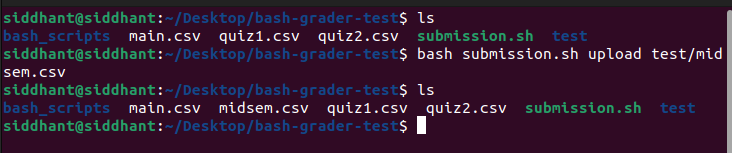
\includegraphics[width=\textwidth]{upload.png}
In the above example, the file \verb"quiz1.csv" is uploaded i.e. copied into the current directory from the filepath given as argument by the user.
The script checks if the file exists and if it is a csv file. If it is, only then is the file copied into the current directory.\\
\textbf{Script files : upload.sh }


\subsection{Total}
\begin{center}
    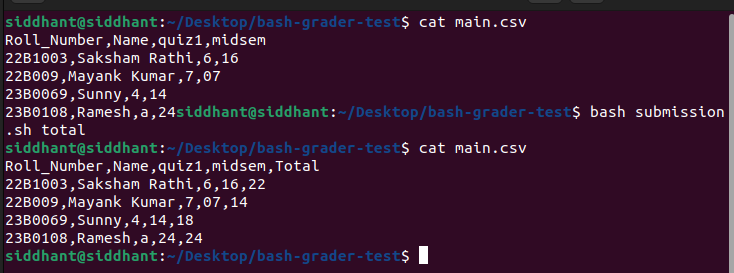
\includegraphics[width=10cm]{total.png}
\end{center}
In the above example, the script totals the marks of each student over all exams and adds a new column \verb"Total" to the \verb"main.csv" file.
If the marks column has \verb"a" as its entry, the script skips that row while totaling.\\
\textbf{Script files : total.awk }

\subsection{Combine}
In the below example, the script combines all the csv files in the current directory into a single \verb"main.csv" file. The script checks if the file is a csv file and if it is not the \verb"main.csv" file.\\ \verb"main.csv" is constructed from scratch in the following steps:
\begin{enumerate}
    \item First, an array of all unique roll numbers and names is created.
    \item Then, based on the exam files, a header is created with the roll numbers and names.
    \item A mesh of \verb"a"'s is created with the dimensions of the header.
    \item Then the script iterates over all exam files and fills in the marks of each student in the mesh, whenever they are found. This ensures that anyone who is not present in a particular exam file is marked as \verb"a"(absent) in \verb"main.csv" for that particular exam.
\end{enumerate}
\begin{figure}[h]
    \begin{subfigure}{0.5\textwidth}
    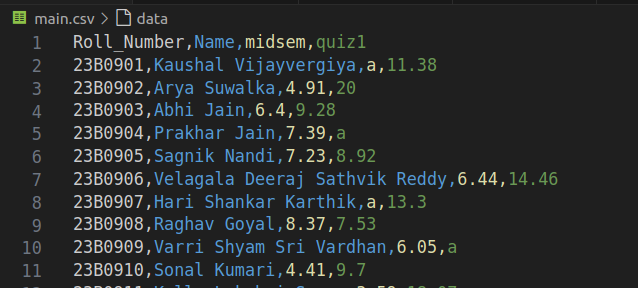
\includegraphics[width=\linewidth, height=3cm]{before_combine.png} 
    \caption{Before combine}
    \label{fig:subim1}
    \end{subfigure}
    \begin{subfigure}{0.5\textwidth}
    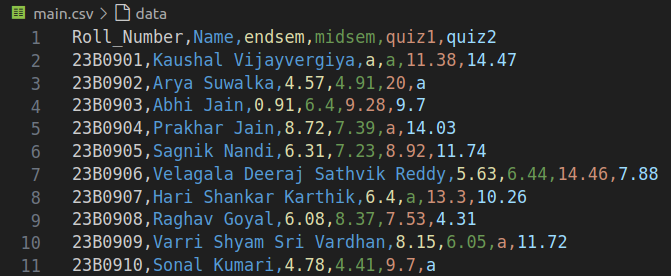
\includegraphics[width=\linewidth, height=3cm]{after_combine.png}
    \caption{After combine}
    \label{fig:subim2}
    \end{subfigure}
\end{figure}

\textbf{Script files : combine.sh, combine.awk}


\subsection{Update}
\begin{figure}[h]
    \begin{subfigure}{0.5\textwidth}
    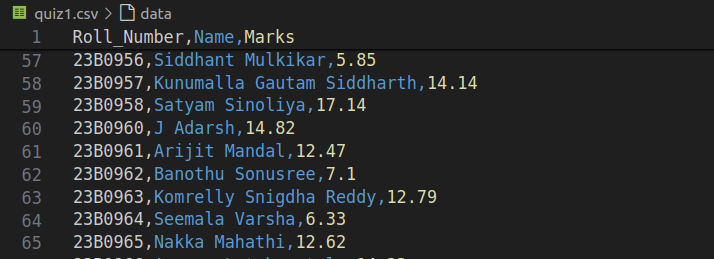
\includegraphics[width=\linewidth, height=3cm]{quiz-before.png} 
    \caption{quiz1.csv before update}
    \end{subfigure}
    \begin{subfigure}{0.5\textwidth}
    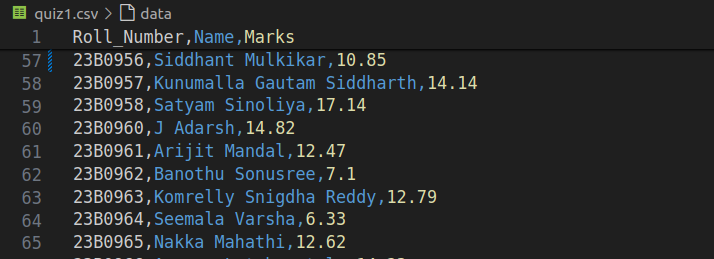
\includegraphics[width=\linewidth, height=3cm]{quiz-after.png}
    \caption{quiz2.csv after update}
    \end{subfigure}
\end{figure}
\begin{figure}[h]
    \begin{subfigure}{0.5\textwidth}
    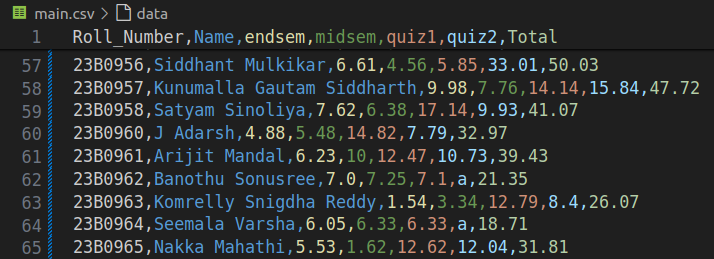
\includegraphics[width=\linewidth, height=3cm]{main-before.png} 
    \caption{main.csv before update}
    \end{subfigure}
    \begin{subfigure}{0.5\textwidth}
    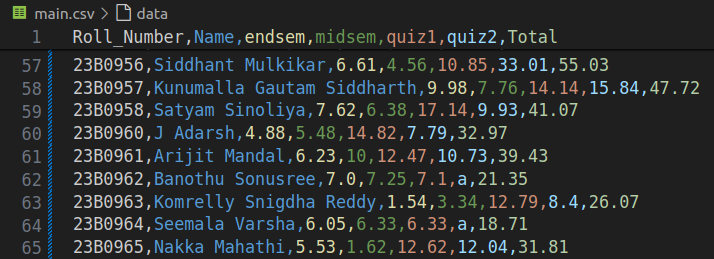
\includegraphics[width=\linewidth, height=3cm]{main-after.png}
    \caption{main.csv after update}
    \end{subfigure}
\end{figure}
In the above example, the script updates the marks of \textbf{23B0956} in \verb"quiz1.csv" and \verb"main.csv".\\
The script first asks the user for the roll number and name of the student whose marks are to be updated. It then checks if the student's name matches with the name paired up with the roll number given by the user. If the names do not match, the script confirms with the user with a prompt for the correct name.\\
It then checks if the student is present in the \verb"main.csv" file and if the exam file exists. If the student is present in the \verb"main.csv" file, the script updates the marks of the student in \verb"main.csv" by calling \verb"update_main.awk" and the exam file by calling \verb"update_exam.awk".\\
If the student's record does not exist in the \verb"main.csv" file, the script prompts the user to confirm if they want to add the student's record to an exam file and \verb"main.csv". If the user confirms, the script adds the student's record to the exam file and \verb"main.csv".\\
It also asks the user if they want to update the marks of the student in some other exam and repeats the same process. If the user does not want to update the marks of the student in any other exam, the script checks if \verb"main.csv" had been totaled before. If it was, then the script calls \verb"total.awk" to correct the total, as the marks in \verb"main.csv" have been updated.\\

\textbf{Script files : update.sh, update\_exam.awk, update\_main.awk, total.awk} 

\subsection{Rank}
This commands takes the examname as a command line argument and ranks the students based on the marks in that exam.
If the user enters \verb"main" as the examname, the script ranks the students based on the total marks in \verb"main.csv". The ranked marklists are sorted according to rank and are stored in the folder \verb"ranked_marklists" in the current directory.\\

\textbf{Script files : rank.sh }

\subsection{Git Init}
This command initializes a remote git repository at the path given by the user as a command line argument.\\
It also checks if the path given is a valid path. If a remote repository is already initialized for the current directory, the script prompts the user to confirm if they want to reinitialize the repository.
If the user confirms, the script reinitializes a fresh remote repository at the path provided by the user.\\ 

It also creates a hidden folder \verb".gitrepo" in the current directory. This folder contains a hidden file \verb".gitreponame" which stores the name of the remote repository and \verb".git_log" which records the commit history.\\

Apart from initialization, the script also copies all the csv files in the current directory at the time of initialization to a hidden folder \verb".ogfiles" in the remote repository. The \verb".ogfiles" folder contains the first version of every file which was ever committed. This serves as a refernce point for all files, for my \textbf{diff patch} system for \verb"git\_checkout" to work.\\

\textbf{Script files : git\_init.sh}
\subsection{Git Add}
This command first checks if a remote repository has been initialized for the current directory. If it has not, the script prompts the user to initialize a remote repository first.\\
This command then prompts the user to enter all the files, which they want to add to the staging area, separated by spaces. It then copies all the files to the staging area in the remote repository. If any particular file doesnt exist in the current directory, it gives an error message.\\
\textbf{Script files : git\_add.sh}

\subsection{Git Remove}
This command first checks if a remote repository has been initialized for the current directory. If it has not, the script prompts the user to initialize a remote repository first.\\
It then prompts the user to enter all the files, which they want to remove from the staging area, separated by spaces. It then deletes all the files from the staging area in the remote repository. If any particular file doesnt exist in the staging area, it gives an error message.\\

\textbf{Script files : git\_remove.sh}

\subsection{Git Commit}
The command first checks if a remote repository has been initialized for the current directory. If it has not, the script prompts the user to initialize a remote repository first.\\
It then checks what all files in the staging area are modified with respect to the \textbf{first version of the file} in the \verb".ogfiles" folder. It also checks for any new files which were created and committed for the first time. It then updates the \verb".git_log" file with these modified and added files, along with the commit message and the files which were modified or added in this commit, which is uniqely identified by the commit message, given by the user and the 16 character hash commit id, generated randomly using the \verb"uuidgen" command. A folder with the commit-id as its name is created in the commits folder of the remote repository.\\

If any file in the staging area is not present in the \verb".ogfiles" folder, it adds it to the \verb".ogfiles" folder.\\ It then copies the diff of the file from the \verb".ogfiles" folder and the file in the staging area into the commit-id folder.\\

It also gets the list of all csv files in the current repository at the time of the commit and stores their name in a hidden \verb".files" file in the commit-id folder. This provides a snapshot of all the files in the current repository at the time of the commit, which is useful at the time of \verb"git\_checkout".The stage is deleted after the commit is made.\\

\textbf{Script files : git\_commit.sh}

\subsection{Git Checkout}
The command first checks if a remote repository has been initialized for the current directory. If it has not, the script prompts the user to initialize a remote repository first.\\
The user can checkout a particular commit by entering the commit-id (even entering the first few characters of the commit-id works too, if they are unique and not shared with any other commit-id) or the commit message. The script then parses and checks for matches to the commit-id or the commit message in the \verb".git_log" file. If it finds a match, it goes to the commit-id folder.//
There, it gets the snapshot of the current repository at the time of the commit from the \verb".files" file. It also gets the list of patch files in the commit-id folder.\\

It deletes all the .csv files from the current directory and then iterates over all files in the snapshot. If the patch file exists for a particular file, it applies \verb"patch -b" command to this patch file and the corresponding file in the \verb".ogfiles" folder, which gives back the version of the file at that commit as \verb"<filename>.csv" and also the original file in the \verb".ogfiles" as \verb"<filename>.csv.orig".
The .csv file is then copied from the \verb".ogfiles" folder to the current directory and the .csv.orig file is renamed to .csv file, hence restoring the original file in the \verb".ogfiles" folder.\\

\textbf{Script files : git\_checkout.sh}

\subsection{Git Log}
The command first checks if the remote repository has been initialized for the current directory. If it has not, the script prompts the user to initialize a remote repository first.
The script then reads the \verb".git_log" file and prints the commit history log in a readable format, with the commit-id, commit-message and time of commit. It also displays any new files created in the current directory, when they are committed for the first time, by the name \textbf{New files added:}, and if any files were modified from the time when the time the remote repository was initialized, it also shows them under the name \textbf{Files modified:} \\

While this command only displays the commit history log, it is actually the \verb"git_commit" command which actually updates the \verb".git_log" file, at every commit.\\

\textbf{Script files : git\_log.sh}
\subsection{Git head}
This command shows the present head of the current directory.\\

\textbf{Script files : git\_head.sh}


\subsection{Graphs}
This command calls the \verb"graphs.py" python script, which has a interface where users can choose between a histogram and a scatter plot. Then, the user can choose between a particular exam or \verb"main" (for \verb"main", it considers the total marks for mark generation). It then calls the corresponding function from \verb"graph_functions.py" to plot the graph, if the csv file of the exam exists.\\
The graphs also show the demarcation for 90th percentile, 75th percentile and mean marks.\\

\textbf{Modules used for graph generation: os, csv, matplotlib}\\

\textbf{Script files: graphs.py, graph\_functions.py}

\begin{figure}[h]
    \begin{subfigure}{0.5\textwidth}
    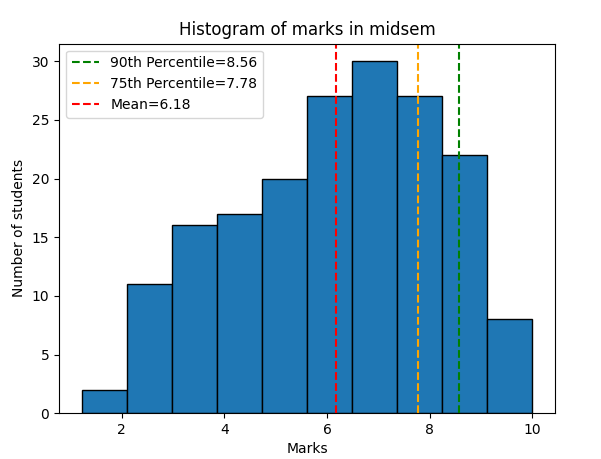
\includegraphics[width=\linewidth, height=5cm]{histogram.png} 
    \caption{Histogram for midsem marks}
    \end{subfigure}
    \begin{subfigure}{0.5\textwidth}
    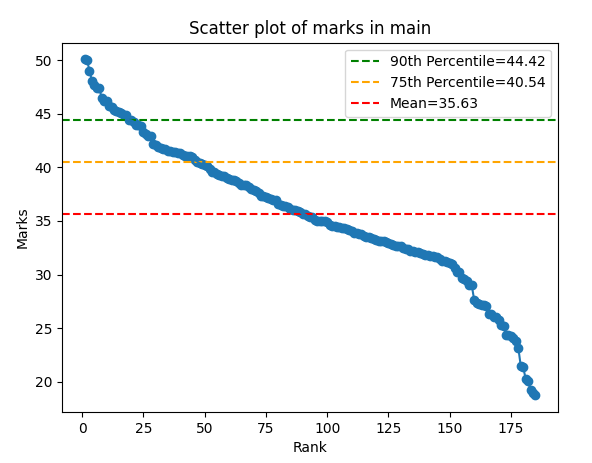
\includegraphics[width=\linewidth, height=5cm]{scatter-plot.png}
    \caption{Scatter plot for main.csv}
    \end{subfigure}
\end{figure}
\newpage

\subsection{Stats}
This command calls the \verb"stats.py" python script, which has a interface where users can choose between a particular exam or \verb"main" (for \verb"main", it considers the total marks for mark generation). It then displays the stats for that particular exam or \verb"main", if the csv file for the exam exists.\\
The stats include the mean, median, mode, standard deviation, $25^{th}$ percentile, $75^{th}$ percentile, $90^{th}$ percentile and maximum marks.\\
All these stats are calculated by calling their respective functions from \verb"stats_functions.py".\\

\textbf{Modules used for stats generation: os, csv, statistics}\\

\textbf{Script files: stats.py, stats\_functions.py}\\
\begin{center}
    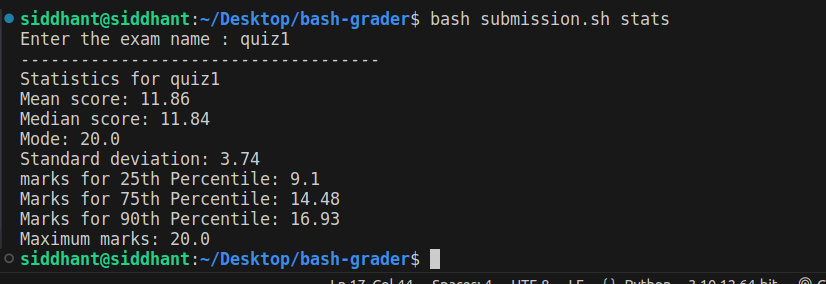
\includegraphics[height=5cm,width=10cm]{stats.png}
\end{center}

\subsection{Report Card}
This command calls the \verb"report_card.py" python script, which has a interface where users can choose between a particular student or all students. It then displays the report card for that particular student or saves the pdf of all student report cards in the \verb"report_cards" folder in the current directory.\\

It gets the grades and percentile rubrics for the grades from the instructor by calling functions from the \verb"grade.py" script. It then gets all the exams conducted and the maximum marks scored in each of these exams. Student marks for all students are also fetched by using the module \verb"csv".\\ It then calculates the weighted percentage of each student by using the formula:
\begin{equation}
    W.P. = \frac{\sum_{i=1}^{n} {M_i} \times {M_{max_i}}}{\sum_{i=1}^{n} {M_{max_i}}^2} \times 100\\
\end{equation}
where $M_i$ is the marks scored by the student in exam i, $M_{max_i}$ is the maximum marks scored in exam i and $n$ is the number of exams.\\

This is considering the maximum marks scored in each exam as the total marks for that exam. This ensures that a person with more marks in an exam with a greater weightage gets a higher weighted percentage.\\

The script then calculates the grade of each student by using the weighted percentage and the rubrics provided by the instructor. Then the percentiles of each student are calcualted with this weighted percentage using the \verb"scipy" module.
Then, the report card is generated from a template report card and text is put on the template using the \verb"PIL" module and then converted to pdf form for all students, while it's only displayed for one person.

\begin{center}
    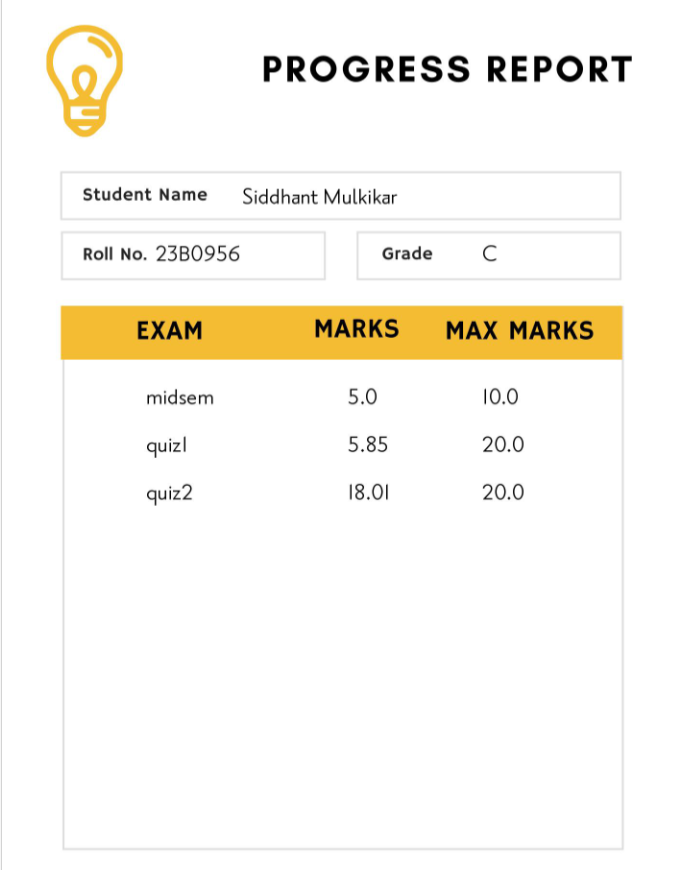
\includegraphics[height=10cm,width=8cm]{report-card.png}
\end{center}

\textbf{Modules used for report card generation: os, csv, statistics, scipy, PIL}\\

\textbf{Script files: report\_card.py, grade.py}

\begin{thebibliography}{9}

\bibitem{bash}Bash manual: \url{https://www.gnu.org/software/bash/manual/bash.html}
\bibitem{awk} Awk manual: \url{https://www.gnu.org/software/gawk/manual/gawk.html}
\bibitem{python} Python manual: \url{https://docs.python.org/3/}
\bibitem{matplotlib}Matplotlib manual:  \url{https://matplotlib.org/}
\bibitem{scipy}Scipy module: \url{https://www.scipy.org/}
\bibitem{PIL}PIL module:  \url{https://pillow.readthedocs.io/en/stable/}
\bibitem{csv}csv module: \url{https://docs.python.org/3/library/csv.html}
\bibitem{os}os module:  \url{https://docs.python.org/3/library/os.html}

\end{thebibliography}

\end{document}

